\section{Dettagli Implementativi}

\begin{frame}{Le Fasi}
  \begin{table}
    \renewcommand\arraystretch{1.4}\arrayrulecolor{LightSteelBlue3}

    \begin{tabular}{@{\,}r <{\hskip 2pt} !{\foo} >{\raggedright\arraybackslash}p{5cm}}

      \addlinespace[1.5ex]
      Introduzione     & \small{fase inziale}                                                      \\
      Proposte Attive  & \small{I cittadini possono avanzare proposte}                             \\
      Votazione        & \small{I cittadini votano le proposte  }                                  \\
      Analisi Proposte & \small{L'azienda considera le proposte}                                   \\
      Bilancio         & \small{Viene stanziato un bilancio }                                      \\
      Risultati        & \small{I bilanci vincitori vengono implementati e i cittadini aggiornati} \\
      % \multicolumn{1}{c!{\bfoo}}{} &
    \end{tabular}
  \end{table}
\end{frame}
\begin{frame}{Autenticazione}
  Decidim supporta la gestione dei permessi per i singoli componenti/fasi

  Una di queste prende il nome di \emph{Verifica delle autorizzazioni}

  \begin{wrapfigure}{r}{0.50\textwidth}
    \centering
    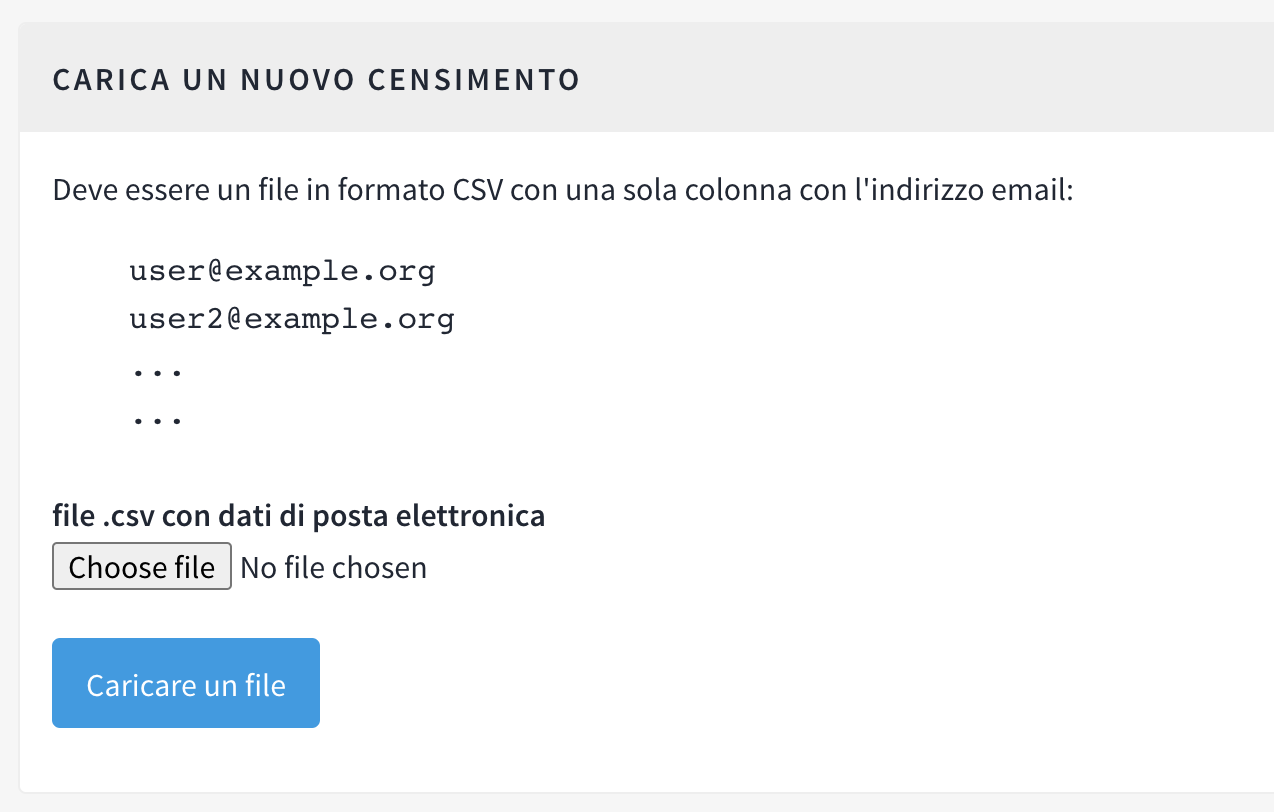
\includegraphics[width=0.50\textwidth]{images/auth}
  \end{wrapfigure}

  Per gestire l'autenticazione si potrebbe importare all'interno di Decidim una lista di mail possedute dall'azienda.

  (ad esempio quelle registrate all'interno degli "sportelli" online dell'azienda e quindi validate)

\end{frame}